\section{From Weighted Model Counting to Tensor Networks}
\label{sec:tensors:wmc}
In this section, we introduce a framework for solving the problem of weighted model counting with tensor networks. The task in weighted model counting is to count the total weight, subject to a given (literal) weight function, of the set of solutions of input constraints. Formally:
\begin{definition}[Weighted Model Count]
  Let $\varphi$ be a formula over Boolean variables $X$ and let $W: X \times \{0,1\} \rightarrow \mathbb{R}$ be a function (called the \emph{weight function}). The \emph{weighted model count} of $\varphi$ w.r.t. $W$ is
  $$W(\varphi) \equiv \sum_{\tau \in \domain{X}} \varphi(\tau) \cdot \prod_{x \in X} W(x, \tau(x)).$$
\end{definition}


% Let us first define weighted model counting. Recall that a \emph{weight function} over a set of variables $X$ is a function $W$ that assigns a (real) weight to the literals $x$ and $\neg x$ for each $x \in X$. The \emph{weight} of a model $\tau \subseteq X$ is the product of the weights of all satisfied literals, and the 

% : X \cup \neg X \rightarrow \mathbb{R}$, where $\neg X = \{\neg x~:~x \in X\}$.


% For example, consider the reduction from constrained counting to tensor network contraction \cite{BMT15}. Recall that the \emph{model count} of a formula $F$ (defined over a set of propositional variables $X$) is the number of subsets of $X$ on which $F$ evaluates to true. There is a polynomial-time algorithm to construct a tensor network whose contraction is the model count of an input formula $F$. 

Note that $[X]$ is the set of all functions $\tau$ from $X$ to $\{0, 1\}$. If $W$ is the constant function that always returns 1, $W(\varphi)$ is known as the \emph{unweighted model count} of $\varphi$. Existing reductions from model counting to tensor-network contraction \cite{BMT15,KCMR18} focus on unweighted model counting. Since we are interested in the more general problem of weighted model counting, we prove that the reduction can be easily extended:
\begin{theorem}
\label{thm:wmc-reduction}
Let $\varphi$ be a CNF formula over Boolean variables $X$ and let $W$ be a weight function. One can construct in polynomial time a tensor network $N_\varphi$ such that $\tnfree{N_\varphi} = \emptyset$ and the contraction of $N_\varphi$ is $W(\varphi)$.
\end{theorem}
\begin{proof}
The key idea is to include in $N_\varphi$ a tensor $A_x$ for each variable $x \in X$ and a tensor $B_C$ for each clause $C \in \varphi$ such that the tensors share an index if and only if the corresponding variable appears in the corresponding clause.

For each $C \in \varphi$, let $\support{C}$ be the set of Boolean variables that appear in $C$. Similarly, for each $x \in X$, let $\depend{x}$ be the set of clauses that contain $x$. Define $I = \{(x, C) : C \in \varphi, x \in \support{C}\}$ to be a set of indices, each with domain $\{0, 1\}$. That is, $I$ has an index for each appearance of each variable in $\varphi$.

For each $x \in X$, let $A_x: [\{x\} \times \depend{x}] \rightarrow \mathbb{R}$ be the tensor defined by $$A_x(\tau) \equiv \begin{cases}W(x, 1)&\text{if}~\tau((x,C)) = 1~\text{for all}~C \in \depend{x}\\W(x, 0)&\text{if}~\tau((x,C)) = 0~\text{for all}~C \in \depend{x}\\0&\text{otherwise.}\end{cases}$$

Next, for each $C \in \varphi$, let $B_C: [\support{C} \times \{C\}] \rightarrow \mathbb{R}$ be the tensor defined by
$$B_C(\tau) \equiv \begin{cases}1& \text{if}~\{x: x \in \support{C}~\text{and}~\tau((x, C)) = 1\}~\text{satisfies}~C\\0&\text{otherwise.}\end{cases}$$

Finally, let $N_\varphi = \{ A_x : x \in X\} \cup \{B_C : C \in \varphi\}$. Each index $(x, C) \in I$ appears exactly twice in $N_\varphi$ (in $A_x$ and $B_C$) and so is a bond index. Thus $N_\varphi$ is a tensor network with $\tnfree{N_\varphi} = \emptyset$. We now compute $\tntensor{N_\varphi}$, the contraction of $N_\varphi$. By Definition 5,
$$\tntensor{N_\varphi}(\emptyset) = \sum_{\rho \in \domain{I}} \prod_{x \in X} A_x(\rho\restrict{\{x\} \times \depend{x}}) \cdot \prod_{C \in \varphi} B_C(\rho\restrict{\support{C} \times \{C\}}).$$

To compute the term of this sum for each $\rho \in \domain{I}$, we examine if there exists some $\tau_\rho \in \domain{X}$ such that $\rho((x, C)) = \tau_\rho(x)$ for all $(x, C) \in I$. If so, then by construction $A_x(\rho\restrict{\{x\} \times \depend{x}}) = W(x, \tau_\rho(x))$ and $B_C(\rho\restrict{\support{C} \times \{C\}}) = C(\tau_\rho\restrict{\support{C}})$. On the other hand, if no such $\tau_\rho$ exists then there is some $y \in X$ such that $\rho$ is not constant on $\{y\} \times \depend{y}$. Thus by construction $A_y(\rho\restrict{\{y\} \times \depend{y}}) = 0$ and so the term in the sum for $\rho$ is 0. Hence
$$\tntensor{N_\varphi}(\emptyset) = \sum_{\tau \in \domain{X}} \prod_{x \in X} W(x, \tau(x)) \cdot \prod_{C \in \varphi} C(\tau\restrict{\support{C}}) = W(\varphi).$$\hfill$\square$
\end{proof}

\begin{figure}[t]
	\centering
	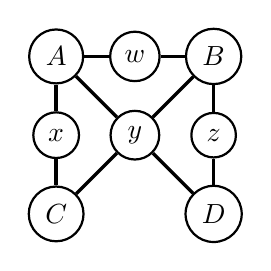
\begin{tikzpicture}
\begin{scope}[every node/.style={circle,thick,draw}]
    \node (C) at (-1,-1) {$C$};
    \node (x) at (-1,0) {$x$};
    \node (A) at (-1,1) {$A$};
    \node (y) at (0,0) {$y$};
    \node (w) at (0,1) {$w$};
    \node (D) at (1,-1) {$D$};
    \node (z) at (1,0) {$z$};
    \node (B) at (1,1) {$B$};
\end{scope}

\begin{scope}[every node/.style={fill=white,circle},
              every edge/.style={draw=black,very thick}]
    \path [-] (A) edge (w);
    \path [-] (A) edge (x);
    \path [-] (A) edge (y);
    \path [-] (B) edge (w);
    \path [-] (B) edge (y);
    \path [-] (B) edge (z);
    \path [-] (C) edge (x);
    \path [-] (C) edge (y);
    \path [-] (D) edge (y);
    \path [-] (D) edge (z);
\end{scope}
\end{tikzpicture}
	\hspace{1cm}
	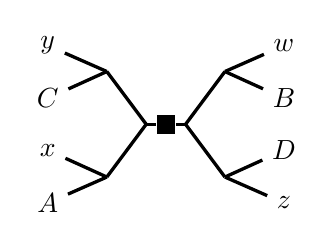
\begin{tikzpicture}
%\begin{scope}[every node/.style={circle,thick,draw}]
    \node (y) at (-1.5,1) {$y$};
    \node (C) at (-1.5,0.33) {$C$};
    \node (x) at (-1.5,-0.33) {$x$};
    \node (A) at (-1.5,-1) {$A$};
    
    \node (w) at (1.5,1) {$w$};
    \node (B) at (1.5,0.33) {$B$};
    \node (D) at (1.5,-0.33) {$D$};
    \node (z) at (1.5,-1) {$z$};
%\end{scope}
    \node (yC) at (-0.75, 0.67) {};
    \node (xA) at (-0.75, -0.67) {};
    \node (wB) at (0.75, 0.67) {};
    \node (zD) at (0.75, -0.67) {};
    
    \node (yCxA) at (-0.25, 0) {};
    \node (wBzD) at (0.25, 0) {};

\begin{scope}[every node/.style={fill=black,rectangle}]
    \node (root) at (0, 0) {};
\end{scope}
    
\begin{scope}[every node/.style={fill=white,circle},
              every edge/.style={draw=black,very thick}]
    \path [-] (y) edge (yC.center);
    \path [-] (C) edge (yC.center);
    \path [-] (x) edge (xA.center);
    \path [-] (A) edge (xA.center);
    \path [-] (w) edge (wB.center);
    \path [-] (B) edge (wB.center);
    \path [-] (z) edge (zD.center);
    \path [-] (D) edge (zD.center);
    
    \path [-] (yC.center) edge (yCxA.center);
    \path [-] (xA.center) edge (yCxA.center);
    \path [-] (wB.center) edge (wBzD.center);
    \path [-] (zD.center) edge (wBzD.center);
    
    \path [-] (yCxA.center) edge (root);
    \path [-] (wBzD.center) edge (root);
\end{scope}
\end{tikzpicture}
	\caption{\label{fig:wmc-example} The tensor network (left) produced by Theorem \ref{thm:wmc-reduction} on $\varphi = (w \lor x \lor \neg y) \land (w \lor y \lor z) \land (\neg x \lor \neg y) \land (\neg y \lor \neg z)$, consisting of 8 tensors and 10 indices. Vertices in this diagram are tensors, while edges indicate that the tensors share an index. The weight function affects the entries of the tensors for $w$, $x$, $y$, and $z$. This tensor network has a contraction tree (right) of max rank 4, but no contraction trees of smaller max rank.}
\end{figure}

See Figure \ref{fig:wmc-example} for an example of the reduction. This reduction is closely related to the formulation of model counting as the marginalization of a factor graph representing the constraints. Unlike the reduction to factor-graph marginalization, which only assigns factors to clauses, we must also assign a tensor to each variable $x$. For example, if $x$ has weights $W(x, 0) = W(x,1) = 1$ then the tensor assigned to $x$ is a copy tensor. This reduction can also be extended beyond OR clauses to other types of constraints (e.g. parity or cardinality constraints). 

Theorem \ref{thm:wmc-reduction} suggests that the weighted model count of $\varphi$ can be computed by constructing and contracting $N_\varphi$. We present this framework as Algorithm \ref{alg:wmc}. Algorithm \ref{alg:wmc} is a fixed-parameter algorithm for model counting, parameterized by carving-width of the incidence graph. The existence of such algorithms is easily implied by fixed-parameter algorithms for model counting parameterized by treewidth \cite{FMR08,SS10} since treewidth is bounded by thrice the carving width \cite{sasak10}. A variety of methods can be used in Step 2 to find a contraction tree to contract $N_\varphi$, including the methods \textbf{LG} and \textbf{FT} that we discuss in the following sections.

\begin{algorithm*}[t]
    \label{alg:wmc}
    \caption{Computing the weighted model count with a TN}
    \DontPrintSemicolon
    \KwIn{$\varphi$: A CNF formula}
    \KwIn{$W$: a weight function}
    \KwOut{$W(\varphi)$, the weighted model count of $\varphi$ w.r.t. $W$}
    $N_\varphi \gets \text{tensor network constructed via Theorem \ref{thm:wmc-reduction}}$\;
    $T \gets \func{FindContractionTree}(N_\varphi)$ \tcc*{e.g., \textbf{LG} or \textbf{FG}}
    \Return{$\func{Contract}(N_\varphi,~T)$}
\end{algorithm*}

% Nevertheless, on many benchmarks the carving width of the incidence graph is smaller than the treewidth. Since the width is in the exponent of the running time of decomposition-based counting algorithms, even a small decrease in width can dramatically decrease the running time.


